\usepackage[magyar]{babel}
\usepackage[T1]{fontenc}
\usepackage[utf8]{inputenc}
\usepackage{graphicx}
\usepackage{listings}
\usepackage{amsmath}
\usepackage{amssymb}
%\usepackage{amsthm}
\usepackage{ae,aecompl}

\usetheme{Goettingen}
%\usetheme{Singapore}

%\theoremstyle{plain}
\newtheorem{thm}{Tétel}[section]
\newtheorem{thmsub}{Tétel}[subsection]
\newtheorem{lem}[thm]{Lemma}
\newtheorem{lemsub}[thmsub]{Lemma}
\newtheorem{all}[thm]{Állítás}
\newtheorem{allsub}[thmsub]{Állítás}
\newtheorem{kov}[thm]{Következmény}
\newtheorem{sej}[thm]{Sejtés}

%\theoremstyle{definition}
\newtheorem{defn}[thm]{Definíció}
\newtheorem{defnsub}[thmsub]{Definíció}
\newtheorem{jel}[thm]{Jelölés}

%\theoremstyle{remark}
\newtheorem{alg}[thm]{Algoritmus}
\newtheorem{megj}[thm]{Megjegyzés}
\newenvironment{biz}{Bizonyítás: }{$\square$}
\newcommand{\leftexp}[2]{{\vphantom{#2}}^{#1}{#2}}

\title{Algoritmusok 3 dimenziós D-szimbólumokra}
\author{Boróczki Lajos}
\date{2011. február 15.}

\begin{document}

\begin{frame}
  \maketitle
\end{frame}

\begin{frame}
  \mode<presentation>{\frametitle{Kivonat}}
  \tableofcontents
\end{frame}
\newpage

\section{Bevezetés}
\begin{frame}
  Bevezetés:
  \begin{itemize}
    \item Algebrai leírás a baricentrikus felbontás segítségével
    \item Szükséges feltételek
    \item A feltételeknek megfelelő leírások felsorolása
    \item A kapott leírások elemzése
    \item Alapvető irány: hogyan kapunk kövezést egy adott leírásból
  \end{itemize}
\end{frame}

\section{Kövezésből D-szimbólum}
\begin{frame}
  D-szimbólum felépítése általánosan:
  \begin{itemize}
    \item Tetszőleges geometria tetszőleges kövezése leírható D-szimbólumok
      segítségével. \mode<article>{A D-szimbólumok a szomszédsági viszonyokat
      írják le egy $d+1$ színű multigráf és egy mátrixfüggvény segítségével.}
    \item Baricentrikus felbontás. \mode<article>{Vegyük a kövezés baricentrikus
      felbontását, ami egy síkbeli háromszögelés általánosítása a $d$ dimenziós
      térre. A baricentrikus felbontást úgy kapjuk a kövezés kompakt
      alaptartományából, hogy az alaptartománynak vesszük a testközéppontját,
      majd egy $d-1$ dimenziós lap középpontját, ezen a lapon egy $d-2$
      dimenziós él középpontját, stb. (Ez a felbontás a lehetséges zászlókkal is
      leírható lenne.) Ezt a szimpliciális térkitöltést jelöljük
      $\mathcal{C}$-vel.}
    \item Szomszédsági operációk. \mode<article>{Következő lépésként bevezetünk
      szomszédsági operációkat az előbb előállított baricentrikus szimplexekre:
      $\sigma_0,\sigma_1,\ldots,\sigma_d.$ Az operációk jelentése: $\sigma_i(C)$
      a $C\in \mathcal{C}$ szimplex azon szomszédja, amely az $i$-lapja, azaz az
      $i$. csúccsal szemközti lap mentén szomszédos $C$-vel.  Minden $\sigma_i$
      operáció egy involúció a fent leírt szimplexek $\mathcal{C}$ halmazán.}
      Jelölés:\\<all>
\setlength{\unitlength}{1cm}
$\sigma_0$:
\begin{picture}(1,0.2)
  \multiput(0,0.1)(0.2,0){5}{\circle*{0.001}}
\end{picture},
$\sigma_1$:
\begin{picture}(1,0.2)                                                                                 
  \multiput(0,0.1)(0.25,0){4}{\line(1,0){0.15}}                                                        
\end{picture},
$\sigma_2$:
\begin{picture}(1,0.2)
  \put(0,0.1){\line(1,0){1}}
\end{picture},
$\sigma_3$:
\begin{picture}(1.5,0.2)
  \multiput(0,0.1)(0.5,0){3}{\line(1,0){0.2}}
  \multiput(0.35,0.1)(0.5,0){3}{\circle*{0.001}}
\end{picture}
    \item Egybevágóság csoport szerinti szimplex pályák halmaza.
      \mode<article>{Általában megkövetelhetjük, hogy a kövezésnek egy
      egybevágóság csoportja változatlanul hagyja a kövezés kombinatorikus
      struktúráját, így a baricentrikus felbontást is. Vehetjük az egybevágóság
      csoport szerinti szimplex pályák halmazát, ezeken is jól értelmezett lesz
      a szomszédsági operáció.}
    \item $(d-2)$-lap körüli szimplex pályák. \mode<article>{Következő lépésként
      vizsgáljuk meg, hogy egy $(d-2)$-lap körül ($3$ dimenzióban él körül) hány
      baricentrikus szimplex ($\mathcal{M}$ mátrix-függvény értékeinek duplája)
      illetve hány szimplex pálya ($\mathcal{R}$ mátrix-függvény értékek
      duplája) csatlakozik.}
  \end{itemize}
\end{frame}

\subsection{Példa}
\begin{frame}
  Az $\mathbb{E}^3$ tér négyzetes hasábbal történő egyik legegyszerűbb
  térkitöltése. Baricentrikus felbontása és a szimplex pályákhoz tartozó
  multigráf: \mode<article>{\ref{abra:hasab_bari}.
  ábra. Mivel minden szimplex pályára definiálva van minden szomszédsági
  reláció, ezért az áttekinthetőség kedvéért azokat a hurok relációkat nem ábrázoljuk,
  melyek sík tükrözéssel önmagára képezik le a pályát.}
  \begin{figure}
    \mode<article>{\caption{\label{abra:hasab_bari} Piros:1, kék:2, zöld:3}}
    \center
    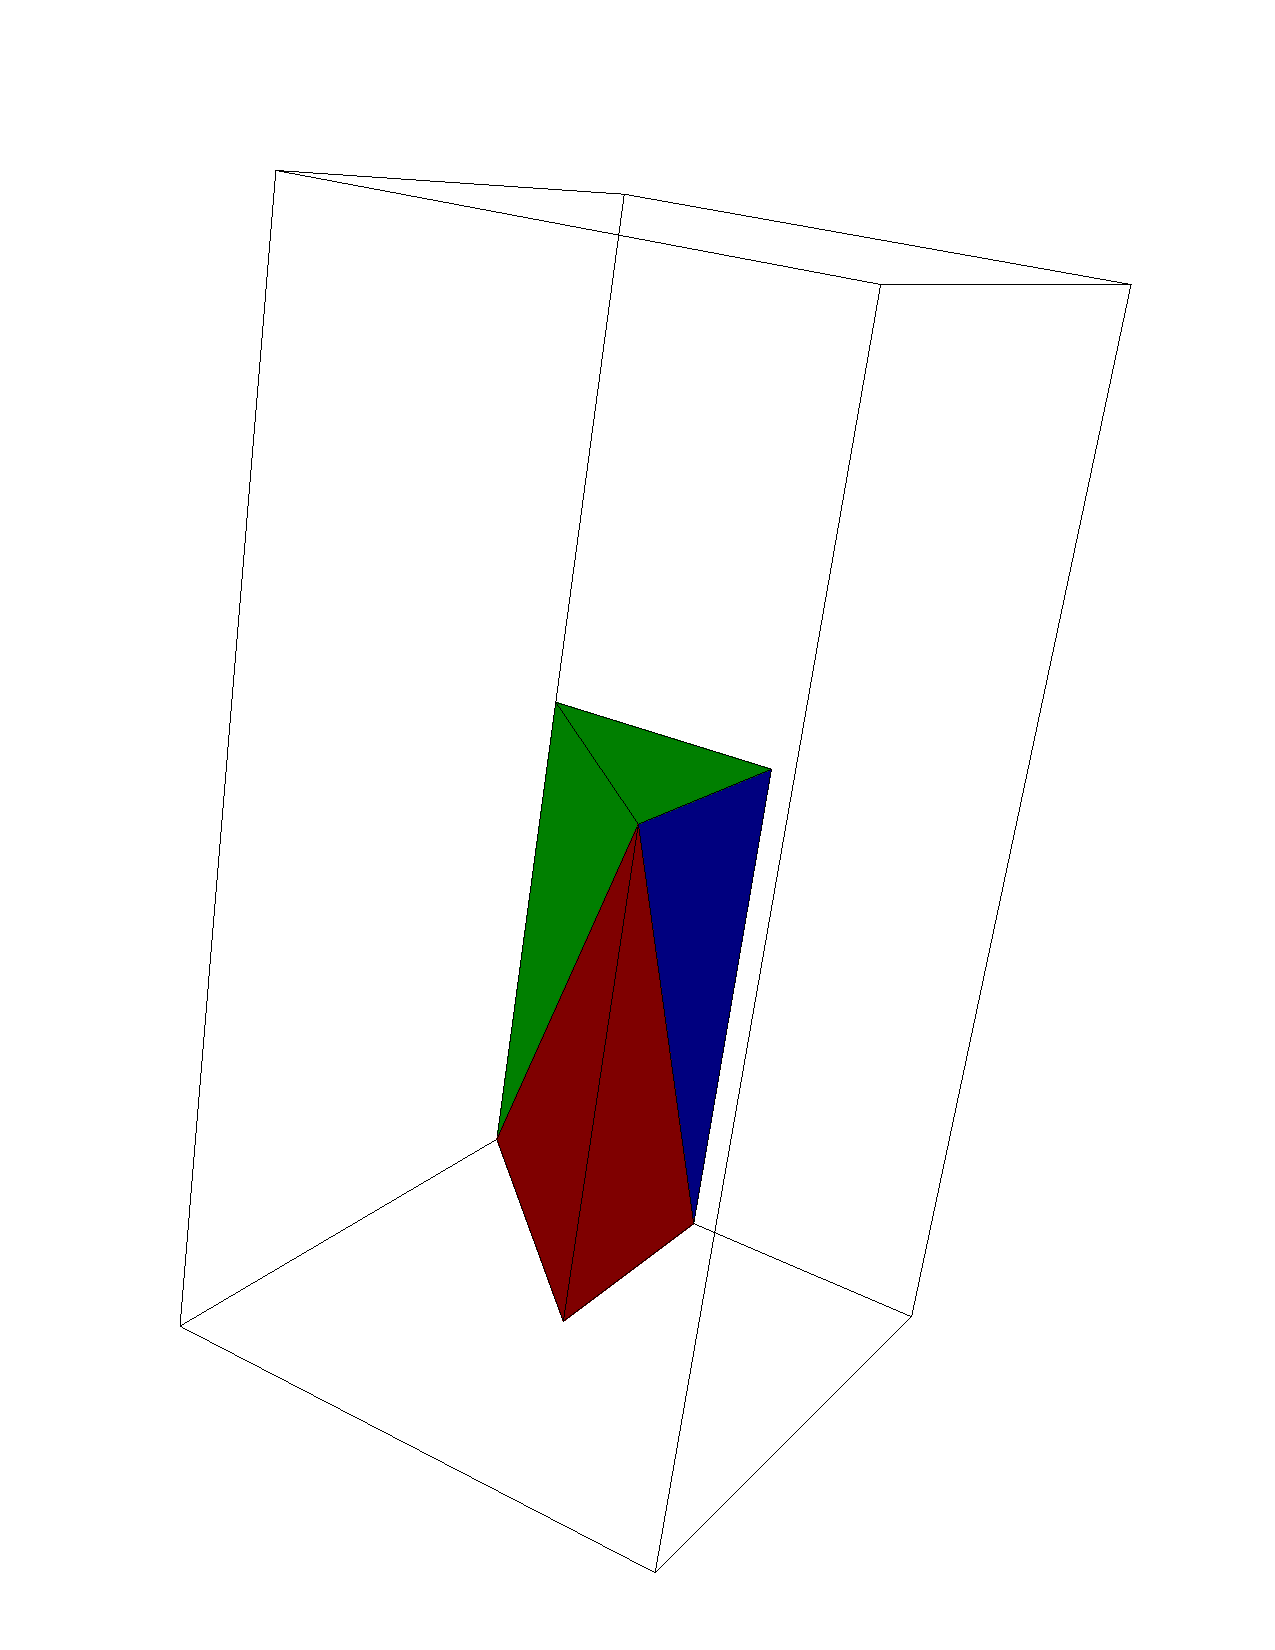
\includegraphics[width=0.4\textwidth]{hasab_bari.pdf}
    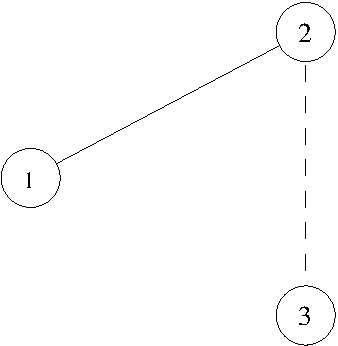
\includegraphics[width=0.35\textwidth]{hasab_D-graf.pdf}
  \end{figure}
\end{frame}

\begin{frame}
  A mátrixfüggvények ($\mathcal{D}$ a szimplex pályák halmaza,
  $D_i\in\mathcal{D}$):
  \begin{equation*}
    \mathcal{R}(D_1)=
    \left(
    \begin{array}{cccc}
      1 & 1 & 2 & 1\\
      1 & 1 & 3 & 1\\
      2 & 3 & 1 & 2\\
      1 & 1 & 2 & 1
    \end{array}
    \right)
  \end{equation*}
  \begin{equation*}
    \mathcal{R}(D_2)=
    \left(
    \begin{array}{cccc}
      1 & 2 & 2 & 1\\
      2 & 1 & 3 & 2\\
      2 & 3 & 1 & 2\\
      1 & 2 & 2 & 1
    \end{array}
    \right)
  \end{equation*}
  \begin{equation*}
    \mathcal{R}(D_3)=
    \left(
    \begin{array}{cccc}
      1 & 2 & 1 & 1\\
      2 & 1 & 3 & 2\\
      1 & 3 & 1 & 1\\
      1 & 2 & 1 & 1
    \end{array}
    \right)
  \end{equation*}

  \begin{equation*}
    \forall D_i\in\mathcal{D}:\;
    \mathcal{M}(D_i)=
    \left(
    \begin{array}{cccc}
      1 & 4 & 2 & 2\\
      4 & 1 & 3 & 2\\
      2 & 3 & 1 & 4\\
      2 & 2 & 4 & 1
    \end{array}
    \right)
  \end{equation*}
\end{frame}

\section{D-szimbólumból kövezés}
\begin{frame}
  D-szimbólumból kövezés:
  \begin{itemize}
    \item \mode<presentation>{Ellenkező irány} \mode<article>{Az eddigiekben
      egy kövezés baricentrikus szimplex-felbontásából jutottunk el a
      D-szimbólum fogalmáig. Mostantól vizsgáljuk az ellenkező irányt.} 
    \item Vegyünk egy diagramot. A diagram csúcsainak halmazát
      $\mathcal{D}$-vel, a rajtuk értelmezett szomszédsági operációk halmazát
      $\Sigma_I$-vel jelöljük. \mode<article>{A diagram csúcsai a különböző
      szimplex pályákat, az élei pedig a szomszédságokat jelölik, a különböző
      szomszédsági operációkat különböző színekkel jelölve ($d$ dimenzióban
      $d+1$ különböző színre van szükségünk.) A diagramot a szomszédsági
      operáció miatt $d+1$ involutív permutációval is leírhatjuk.}
    \item Vegyünk egy a diagram csúcsain értelmezett $\mathcal{M}$
      mátrixfüggvényt.
    \item Milyen szükséges feltételeket kell szabnunk a diagramra és a
      mátrixfüggvényre, hogy az valamely geometriában leírhasson egy értelmes
      egybevágóság-csoportot?
  \end{itemize}
\end{frame}

\subsection{Feltételek}
\begin{frame}
  D-szimbólum: $(\Sigma_I,\mathcal{D},\mathcal{M})$ hármasok. \mode<article>{Az
  alábbi feltételeknek megfelelő $(\Sigma_I,\mathcal{D},\mathcal{M})$ hármasokat
  nevezzük Delone-Delaney-Dress szimbólumnak, röviden D-szimbólumnak.}
  \begin{itemize}
    \item Feltételek D-diagramokra:
      \begin{enumerate}
	\item $\mathcal{D}$ véges
	\item A szimplex pályákon értelmezett szomszédsági operációk involutív
	  permutációk\mode<article>{, vagyis $\forall i\in I, \sigma_i\in
	  \Sigma_I, \forall D\in \mathcal{D}$:
	  \begin{align*}
	    \sigma_i\sigma_i(D)=D 
	  \end{align*}
	  A diagram minden csúcsában az azonos
	  színű élek foka 1 vagy 2. A fok pontosan akkor 2, ha az él egy hurok
	  (kezdő és végpontja azonos.)}
	\item Nem szomszédos operáció-párokat alkalmazva legfeljebb $2$ lépésből
	  visszajutunk a kiindulási csúcsba\mode<article>{. \newline $\forall
	  i,j\in I, \forall D\in \mathcal{D}$:
	  \begin{align*}
	    |i-j|\geq 2 \Rightarrow (\sigma_j\sigma_i)^2(D)=D
	  \end{align*}}
      \end{enumerate}
    \item Bevezetjük a szimplex pályákon (D-diagram csúcsokon) értelmezett $\mathcal{R}$
      mátrix-függvényt\mode<article>{.
	\newline $\forall i,j\in I, \forall D\in \mathcal{D}$:
      \begin{align*}
	r_{ij}(D)=r_{ji}(D)=\mathrm{min}\left\{r\in \mathbb{N}^+|(\sigma_j\sigma_i)^r(D)=D\right\}
      \end{align*}
      A D-diagram feltételei $\mathcal{R}$ mátrix-függvényre vetítve:
      $r_{ii}(D)=1$, illetve $|i-j|\geq 2 \Rightarrow r_{ij}(D)\leq2$}
    \item Feltételek a diagramhoz tartozó $\mathcal{M}$ mátrix-függvényre:
      \begin{enumerate}
	\item Az $\mathcal{R}$ mátrix-függvény minden elemének osztania kell az
	  $\mathcal{M}$ mátrix-függvény megfelelő elemét.
	  \mode<article>{
	  Csak így biztosítható, hogy egy $d-2$ dimenziós lap ($3$ dimenzióban él)
	  teljes körüljárásakor azonos szimplex pályába érkezünk; ami pedig szükséges
	  ahhoz, hogy azonos szimplexbe érkezhessünk. Az $\mathcal{M}$ és
	  $\mathcal{R}$ mátrix-függvények értékeinek hányadosa a kövezés
	  periodicitását mutatja az adott él körül.
	  \newline $\forall i,j\in I, \forall D\in \mathcal{D}$:
	  $r_{ij}(D)|m_{ij}(D)$
	  }
	\item Pálya feltétel\mode<article>{. Minden operáció-párhoz és
	  kiindulási diagram-csúcshoz definiálhatjuk a hozzá tartozó pályát: az
	  összes diagram-csúcs, amit érintünk miközben az operációkat
	  elvégezzük. Az $\mathcal{M}$ mátrix-függvény értékeinek egy-egy pályán belül
	  meg kell egyeznie, különben a kapott kövezésben függne az él körüli
	  szimplexek száma a kezdő szimplextől. A pályát visszafelé bejárva is
	  ugyanazt az utat kell megtennünk, ezért az $\mathcal{M}$
	  mátrix-függvény mátrixai szimmetrikusak.
	  \begin{align*}
	    &\forall i,j\in I, \forall D\in \mathcal{D} \\
	    &\mathcal{D}'=\left\{(\sigma_j\sigma_i)^k(D)|k\in
	    \mathbb{N}\right\}\cup\left\{\sigma_i(\sigma_j\sigma_i)^k(D)|k\in
	    \mathbb{N}\right\}\\
	    &\forall D_1,D_2 \in \mathcal{D}'\\
            &m_{ij}(D_1)=m_{ij}(D_2)=m_{ji}(D_1)=m_{ji}(D_2)
	  \end{align*}
	  }
	\item Az $\mathcal{M}$ mátrix-függvény minden mátrixának főátlójától legalább
	  2 távolságra lévő helyeken $2$-esek állnak\mode<article>{, különben nem
	  kapjuk vissza a baricentrikus felbontást.
	  \newline $\forall i,j\in I, \forall D\in \mathcal{D}$:
	  \begin{align*}
	    m_{ij}(D)=2
	  \end{align*}}
	\item A főátlótól $1$ távolságra lévő helyeken a mátrix-függvény értékei
	  legyenek nagyobbak vagy egyenlőek, mint 2\mode<article>{. Egyenlőség esetén
	  degenerált, illetve mesterkélt esetekhez jutunk, melyekben például
	  digonok is lehetnek lapok. (Szép kövezés esetén egy 3 dimenziós poliéder bármely
	  csúcsában legalább 3 él és 3 lap találkozik, minden lapnak legalább 3
	  oldaléle van, minden élnél legalább 3 test és 3 lap fut össze.)
	  \newline $\forall i\in I-\{0\}, \forall D\in \mathcal{D}$:
	  \begin{align*}
	    m_{i(i-1)}(D)\geq 2
	  \end{align*}}
      \end{enumerate}
  \end{itemize}
\end{frame}

Az eddigi megállapítások szükséges (de nem mindig elégséges)
feltételek olyan $d$ dimenziós (nem feltétlenül euklideszi) térkitöltés
létezésére (amelynek D-szimbóluma $(\Sigma_I,\mathcal{D},\mathcal{M})$.) Most nézzük
speciálisan a 3 dimenziós eset további követelményeit.

\subsection{Rész D-szimbólum}
\begin{frame}
  Rész D-szimbólum:
  \begin{itemize}
    \item Az i-edik komponens vagy rész D-szimbólum
      $(\Sigma_I^i,\mathcal{D}^i,\mathcal{M}^i)$ jelentése\mode<article>{: az i-edik
      operációt elhagyjuk a diagramból illetve a mátrix-függvény soraiból és
      oszlopaiból is.}
    \item A kombinatorikus görbületi függvény számolható\mode<article>{. A rész
      D-szimbólum komponenseihez tartozó kövezésben a D-szimbólum alapján
      felírható a kombinatorikus görbületi függvény:}
      \begin{align*}
	K(\leftexp{c}{\mathcal{D}}^i)=\sum_{D\in
	\leftexp{c}{\mathcal{D}}^i}\left(-1+\sum_{\substack{0\le j<k\le d \\
	j,k\ne i}}\frac{1}{m_{jk}(D)}\right)
	\begin{array}{cccc}
	  > & & S^2 \\
	  = & 0 & \mathbb{E}^2 \\
	  < & & H^2
	\end{array}
      \end{align*}
      \mode<article>{Ez alapján eldönthető, hogy a 3 lehetséges felület közül melyiken valósul
      meg.}
    \item Vizuális jelentés\mode<article>{: A rész D-szimbólum vizuális
      jelentése az adott i-indexű csúcs körüli 1-gyel kisebb dimenziós felületen
      létrehozott $(3-1)$-dimenziós kövezés D-szimbóluma az i-indexű csúcs
      stabilizátora szerint.  Ezért egy i-indexű valódi szimplex-csúcs körüli
      rész D-szimbólum egy szférikus kövezéshez kell tartozzon, egy ideális
      szimplex-csúcs körül euklideszi kövezés alakul ki pl. a hiperbolikus tér
      paraszféra (horoszféra) felületén; a hiperbolikus síkkövezéseket
      kizárjuk, mert modellen kívüli (végtelennél távolabbi) pontot, mint
      i-csúcsot jellemezne.}
    \item Jó orbifold feltétel\mode<article>{: Szférikus síkon történő
      kövezésnek további feltétele, hogy az úgy nevezett  rossz orbifoldokat
      kizárjuk, azaz a következő lehetőségek hibásak (Convay illetve
      Macbeath-féle jelöléseik alapján):
      \begin{align*}
	u=(+,0;[u];\{\}), & & 1<u;\\
	*u=(+,0;[];\{(u)\}), & & 1<u;\\
	uv=(+,0;[u,v];\{\}), & & 1<u<v;\\
	*uv=(+,0;[];\{(u,v)\}), & & 1<u<v.
      \end{align*}
      Ezek a csepp felületekre illetve az észak-déli póluson nem azonosan viselkedő
      gömb felületekre utalnak.}
  \end{itemize}
\end{frame}

\begin{frame}
  További követelmények a rész D-szimbólumok alapján:
  \begin{enumerate}
    \item $(\Sigma_I^1,\mathcal{D}^1,\mathcal{M}^1)$ és
      $(\Sigma_I^2,\mathcal{D}^2,\mathcal{M}^2)$ esetén a
      görbületi függvény pozitív és a jó orbifold feltétel
      teljesül\mode<article>{. Élközépponthoz és lapközépponthoz tartozó
      szimplex csúcs valódi csúcs kell legyen, ezért egy $S^2$-n megvalósuló
      kövezést kell kapjunk.}
    \item $(\Sigma_I^0,\mathcal{D}^0,\mathcal{M}^0)$ és
      $(\Sigma_I^3,\mathcal{D}^3,\mathcal{M}^3)$ esetén a görbületi függvény
      pozitív és a jó orbifold feltétel teljesül, vagy a görbületi függvény
      $0$\mode<article>{. Csúcshoz és test-középponthoz tartozó szimplex csúcs
      lehet valódi, ekkor egy $S^2$-n megvalósuló kövezést kell kapjunk; vagy
      lehet ideális, ekkor $\mathbb{E}^2$-n megvalósuló kövezést kell kapjunk.
      (Az ideális test-középpont esetét a dualitás miatt meghagyjuk; de
      megjegyezzük, hogy a végtelen poliéderekkel történő kövezés nem igazán
      érdekes (egy kisebb dimenziós felület kövezésének felel meg.))}
  \end{enumerate}
\end{frame}


\section{D-szimbólumok felsorolása}
\begin{frame}
  D-szimbólumok felsorolása:
  \begin{itemize}
    \item Nagyravágyó terv\mode<article>{: Az összes $n$-dimenziós geometriában
      az összes lehetséges véges alaptartományú kövezés felsorolásához
      szeretnénk a D-szimbólumokat felhasználni.}
    \item Alapvetően nem tűnik lehetetlennek\mode<article>{, mivel a
      D-szimbólumokat minden olyan kövezésre értelmezhetjük, ahol tudunk
      baricentrikus felbontást végezni.}
    \item Nagyon sok lehetőség van\mode<article>{: a dimenzió és a D-diagram
      elemszámának méretében is exponenciális}
    \item Rendezés a D-diagramokon, algoritmus a felsorolásukra
    \item Rendezés a mátrix-függvényeken, $3$-dimenziós esetben algoritmus a
      lehetséges mátrix-függvények felsorolására \mode<article>{ az előző
      fejezetben felsorolt feltételeknek megfelelően.}
  \end{itemize}
\end{frame}

\subsection{D-diagramok felsorolása}
\begin{frame}
  Rendezés bevezetése a D-diagramokra:
  \begin{itemize}
    \item Bevezetünk egy sorszámozást, ami minden adott kezdőcsúcsú, összefüggő
      D-szimbólum csúcsainak sorszámát megadja\mode<article>{. 
      Legyen $(\Sigma_I,\mathcal{D}(D_1))$ egy D-szimbólum diagramja $D_1$
      kezdőcsúccsal. Számozzuk meg a csúcsokat $1,2,\ldots ,n$ sorszámokkal. 
      $D_1$ sorszáma 1. Tegyük fel, hogy megsorszámoztuk a $D_1,\ldots,D_r$ 
      csúcsokat. A következő csúcs: 
      \begin{enumerate}
	\item Vegyük sorban a $\sigma_0(D_r)$ és $\sigma_1(D_r)$ elmeket, az első,
	  amelyiket még nem sorszámoztuk meg, lesz a következő csúcs.
	\item Ha már sorszámozottak, vegyük sorban
	  \begin{equation*}
	    \sigma_0(D_{r-1}),\ldots,\sigma_0(D_1);\sigma_1(D_{r-1}),\ldots, \sigma_1(D_1)
	  \end{equation*}
	  csúcsokat, az első sorszám nélküli a következő.
	\item Végül ha még mindig nincs meg a következő, vegyük az első
	  sorszámozatlant a következők közül:
	  \begin{equation*}
	    \sigma_2(D_r),\ldots,\sigma_2(D_1); \ldots\ldots; \sigma_d(D_r),\ldots,\sigma_d(D_1)
	  \end{equation*}
      \end{enumerate}

      A diagram összefüggő, ezért minden csúcsát megsorszámozza az algoritmus.
      }
    \item A sorszámozás alapján veszünk egy távolságot\mode<article>{. Bármely
      két elem távolságát meghatározhatjuk úgy, hogy az egyik elemmel indított
      sorszámozás szerint a másik elem sorszámánál 1-el kevesebbet veszünk.
      $D_x$ és $D_y$ távolságának jelölése: $D_xD_y$. Fontos megjegyezni, hogy a
      távolság nem szimmetrikus.}
    \item A csúcsok távolsága alapján veszünk egy rendezést adott kezdőcsúcsú
      diagramok között\mode<article>{. Legyenek $(\Sigma_I,\mathcal{D}(D_1))$ és
      $(\Sigma'_{I'},\mathcal{D}'(D_{1'}))$ két D-szimbólum diagramjai,
      kitüntetett kezdőcsúccsal. Azt mondjuk, hogy $\mathcal{D}<\mathcal{D}'$ a
      következő tulajdonságok alapján:
      \begin{enumerate}
	\item $|I|<|I'|$ (dimenzió)
	\item Ha megegyeznek: $|\mathcal{D}|<|\mathcal{D}'|$ (D-szimbólum elemszáma)                     
	\item Ha egyenlőség áll: $\mathcal{D}$ és $\mathcal{D}'$ elemeinek
	  távolságait hasonlítjuk össze:
	  \begin{itemize}
	    \item $D_1\sigma_d D_1<D_{1'}\sigma_d D_{1'};$ ha egyenlőség áll,
	      $D_2\sigma_d D_2<D_{2'}\sigma_d D_{2'};\ldots;$ ha egyenlőség áll,
	      $D_n\sigma_d D_n<D_{n'}\sigma_d D_{n'}$ ($n-1$-ig is elég menni;)
	    \item Egyenlőség esetén: $D_1\sigma_{d-1} D_1<D_{1'}\sigma_{d-1} D_{1'};
	      \ldots;D_n\sigma_{d-1} D_n<D_{n'}\sigma_{d-1} D_{n'};$
	      \begin{equation*}
		\vdots
	      \end{equation*}
	    \item Egyenlőség esetén: $D_1\sigma_0 D_1<D_{1'}\sigma_0 D_{1'};
	      \ldots;D_n\sigma_0 D_n<D_{n'}\sigma_0 D_{n'}.$
	  \end{itemize}
      \end{enumerate}
      Ha végig egyenlőség állt, a két diagram izomorf.}
  \end{itemize}
\end{frame}

\begin{frame}
  D-diagramokat felsoroló algoritmus:
  \begin{itemize}
    \item Legfeljebb $7$ elemű, $3$-dimenziós D-diagram kevés van
      \mode<article>{a mai számítógépek kapacitásához képest}
    \item Felsoroljuk az összes lehetséges diagramot az összes lehetséges
      sorszámozással
    \item Eldobjuk azokat, amiknél a fenti rendezés szerint van kisebb
  \end{itemize}
\end{frame}

\begin{frame}
  Az összes lehetséges diagramot egy backtrack típusú algoritmussal soroljuk
  fel, aminek működése egy döntési fa teljes bejárásával mutatható be:
  \begin{itemize}
    \item A fa minden csúcsa egy aktuális állapotnak felel meg\mode<article>{, a
      következő adatokat tároljuk:
      \begin{itemize}
	\item Aktuális D-diagram-kezdemény
	\item Vizsgált él adatai: forrásának sorszáma ($1..$elemszám),
	  operációjanak sorszáma ($1..d+1$), céljának sorszáma
	  (forrás$+1..$elemszám)
      \end{itemize}}
    \item Minden csúcsból két irányba tudunk továbbmenni\mode<article>{: hozzáadjuk a
      D-diagram-kezdeményhez a vizsgált élet, vagy nem; és vizsgáljuk a
      következő élet. (A következő élet lexikografikusan vesszük: forrás
      sorszám, operáció sorszám, cél sorszám alapján.)}
    \item A döntési fa levelein ellenőrizzük a diagram szempontjából szükséges
      feltételeket: összefüggő, legkisebb sorszámozás, $\mathcal{R}$
      mátrix-függvény. \mode<article>{Ha a forrás sorszáma egyenlő a diagram
      csúcsainak számával, akkor megnézzük, hogy összefüggő-e a gráf, majd
      előállítjuk az első csúcsot kezdőcsúcsnak vett sorszámozást. Ha ez nem
      ugyanaz, mint az algoritmus által előállított sorszámozás, akkor eldobjuk,
      mert előáll az algoritmus során a jó sorszámozás is. Sorban előállítjuk a
      többi csúcs által generált sorszámozást is, és ha ezek közül bármelyik
      kisebb diagramot ad, akkor eldobjuk, mert előáll a kisebb is.  Végül
      elkészítjük a diagram alapján az $\mathcal{R}$ mátrix-függvényt, és
      megvizsgáljuk, hogy a főátlótól legalább $2$ távolságra levő mezőkben 1-es
      vagy 2-es szerepel-e (csak így lehet az $\mathcal{M}$ mátrix-függvény
      megfelelő helyein 2-es), ha valamelyikben nem az szerepelne, akkor szintén
      eldobjuk a diagramot. Ha idáig eljutottunk, beszúrjuk egy rendezett
      adatrendszerbe (az előbb definiált rendezés szerint.) Ha már szerepelne a
      rendszerben, ez azt jelenti, hogy szimmetrikus a diagram, és egyszer már
      szerepelt. Mivel a későbbiekben a teljes D-szimbólumra is végzünk
      szimmetria ellenőrzést, ezért a diagramot eldobjuk.}
    \item Apró heurisztikák\mode<article>{: A csúcsokban nem adunk hozzá olyan
      élet, ami az involúciót elrontaná; illetve nem lépünk új forrásra anélkül,
      hogy a régi forrásnak lenne legalább $1$ éle (összefüggőség miatt.)}
  \end{itemize}
\end{frame}

\begin{frame}
  Információk D-diagramok alapján:
  \begin{itemize}
    \item Duális: \mode<article>{Ha a szomszédsági operációk sorrendjét
      megfordítjuk, akkor is D-diagramot kapunk (esetleg rossz sorszámozással,)
      mivel szimmetrikusan dolgoztunk (lásd \ref{dual}. ábra.)}
      \begin{figure}
	\mode<article>{\caption{\label{dual} Duális D-diagram pár}}
	\center
	\includegraphics[width=0.4\textwidth]{d3c6_110.pdf}
	\hfill
	\includegraphics[width=0.4\textwidth]{d3c6_182.pdf}
      \end{figure}
    \item Rész D-szimbólumok\mode<article>{: Az egy-egy operáció elhagyásával
      keletkező (akár több komponensű) rész D-szimbólumok összegyűjtése.
      Ez a $3$-dimenziós D-szimbólum követelményeinél válik fontossá.}
  \end{itemize}
\end{frame}

\subsection{Mátrix-függvények felsorolása}
\begin{frame}
  A lehetséges $\mathcal{M}$ mátrix-függvények felsorolásához a következőkre van
  szükség:
  \begin{itemize}
    \item A mátrix-függvények paraméteres előállítása, pályák kezelése\mode<article>{: Azonos
      pályához tartozó szimplex-pár esetén az $\mathcal{M}$
      mátrix-függvény megfelelő értékei meg kell egyezzenek a kövezés
      kombinatorikus struktúrája miatt (különben a szimplexekre és a
      szimplex pályákra ható operációk inkompatibilisek lesznek.) Tudjuk
      továbbá, hogy az $\mathcal{R}$ mátrix-függvény elemeinek osztania kell az
      $\mathcal{M}$ mátrix-függvény elemeit, illetve a nem szomszédos operációk
      esetén az $\mathcal{M}$ mátrix-függvény értéke 2. Így szomszédos
      operációkhoz tartozó pályánként vehetünk egy-egy
      paramétert, amit a megfelelő $\mathcal{R}$ mátrix-függvény elemmel
      szorozva a megfelelő $\mathcal{M}$ mátrix-függvény elemet kapjuk. Itt is
      felléphetnek rossz orbifold esetek, ezeket a rész D-szimbólumok
      vizsgálatával tudjuk megszüntetni (a megfelelő paramétereket azonosnak
      kell választani); ebben az esetben nem csak a szomszédos operációkra kell
      figyelemmel lennünk. A paraméterek minimális értékeit beállítjuk úgy, hogy
      legalább $2$ legyen minden $\mathcal{M}$ mátrix-függvény elem.}
    \item Melyik mátrix-függvényeket tartsuk meg? \mode<article>{Azokat a
      paraméter értékeket tartjuk meg, melyek minden rész D-szimbólum esetén
      megfelelő kombinatorikus görbület-függvényt indukálnak (csúcs és
      testközéppont esetén szférikus vagy euklideszi, lap- és élközéppont esetén
      szférikus.) A paraméterek növelésével a görbület-függvény csökken; így
      ha eljutottunk pl. egy hiperbolikus állapothoz, nem fogunk a paraméterek
      növelésével se euklideszi se szférikus állapotot kapni.}
    \item Bevezetünk egy rendezést az adott D-diagram $\mathcal{M}$
      mátrix-függvényeire is\mode<article>{: Tetszőleges lexikografikus
      rendezést vehetünk.}
  \end{itemize}
\end{frame}

\begin{frame}
  Felsorolás:
  \begin{itemize}
    \item Egy egyszerű felsoroló algoritmus\mode<article>{: A paraméterek
      sorrendje szerinti lexikografikus rendezés szerint vesszük sorba a
      paraméter-rendszereket. Ha az éppen növelt paraméter növelésével elértük a
      megfelelő (euklideszi vagy hiperbolikus) görbületi függvényt, akkor az
      előző paramétert növeljük.}
    \item Ha vannak végtelen láncok, azok optimális kezelése\mode<article>{.
      Végtelen láncok esetén az előző algoritmus nem ér véget, ezért egy kis
      javításra szorul. Észrevehetjük, hogy végtelen paraméter-lánc létezése
      esetén a görbületi-függvény megfelelő $1/m_{ij}$ helyeire $0$-t írva is jó
      értéket ad a függvény. Ezt a tulajdonságot kihasználhatjuk úgy, hogy
      minden éppen aktuális paraméter-rendszer esetén megpróbálunk a minimális
      paraméter-értékek helyére az összes lehetséges módon végtelent írni. Ha ez
      lehetséges, akkor legtöbb végtelent tartalmazó eseteket (részhalmaz
      értelemben legtöbb) megjegyezzük; és olyan esetet már nem vizsgálunk, ahol
      csak ezeket a paramétereket növeljük.}
    \item Átsorszámozással kapunk-e kisebb D-szimbólumot?
      \mode<article>{Szimmetrikus D-diagramok esetén az $\mathcal{M}$
      mátrix-függvény szerinti rendezés esetén nem legkisebb
      paraméter-rendszereket is kiszűrjük.}
    \item Maximális szimmetria csoportú D-szimbólumok kiválasztása a D-szimbólum belső szimmetriája
      alapján\mode<article>{: Szimmetrikusnak akkor nevezünk egy D-szimbólumot,
      ha a D-diagram és az $\mathcal{M}$ mátrix-függvény is szimmetrikus, vagyis
      van olyan átsorszámozhatóság, hogy a két D-szimbólum egyenlő. Ezekben az
      esetekben egy D-morfizmussal kisebb elemszámú D-szimbólumot kapunk.}
  \end{itemize}
\end{frame}

Az eddigiek már megvalósított dolgokról szóltak.

\section{Haladási irány}
\begin{frame}
  Haladási irány:
  \begin{itemize}
    \item Kis kitérő a Schönflies-Bieberbach tétel általánosításának lehetősége
      felé
    \item Folytatjuk a D-szimbólumok realizálhatóságának kérdését a fundamentális
      tartomány előállításával
    \item A fundamentális tartomány alapján felsoroljuk a generátorokat és
      relációkat
    \item Generátorok és relációk alapján splitting keresése
    \item Végül a nagy kérdés, hogy adott D-szimbólum, amiben nincs splitting
      milyen geometriában realizálódik
  \end{itemize}
\end{frame}

\subsection{Schönflies-Bieberbach tétel általánosítása}
\begin{frame}
  Schönflies-Bieberbach tétel általánosítása:
  \begin{itemize}
    \item Schönflies-Bieberbach tétel: $\mathbb{E}^n$ térben minden
      kristálycsoport tartalmaz $n$ lineárisan független eltolást.
      \mode<article>{\newline
      \underline{Definíció}: Az $\mathbb{E}^n$ $n$-dimenziós euklideszi tér
      egybevágóságainak $G$ részcsoportját kristálycsoportnak nevezzük, ha a
      következő feltételek teljesülnek:
      \begin{enumerate}
	\item bármely pont pályája diszkrét
	\item létezik $\mathbb{E}^n$-nek olyan $K$ kompakt részhalmaza, hogy
	  \begin{enumerate}
	    \item $GK=\underset{g\in G}{\bigcup} gK=\mathbb{E}^n$
	    \item $\forall g\in G \setminus \{id\}$ igaz, hogy $\mathrm{int}K \bigcap \mathrm{int}(gK)=\emptyset$
	  \end{enumerate}
      \end{enumerate}
      \underline{Schönflies-Bieberbach tétel}: Ha $G$ az $\mathbb{E}^n$
      $n$-dimenziós euklideszi tér kristálycsoportja, akkor teljesülnek a
      következők:
      \begin{enumerate}
	\item A $G$ csoport tartalmaz $n$ számú lineárisan független eltolást,
	  melyek egy $n$-dimenziós $L$ rácsot alkotnak.
	\item A $dG$ csoport véges. ($dg$ a $g$ egybevágóság lineáris,
	  ortogonális része; $dG=\left\{dg:g\in G\right\}$.)
      \end{enumerate}
      }
    \item A tétel általánosabban átfogalmazható úgy, hogy homogén $n$-dimenziós
      geometriában minden maximális szimmetria-csoportú kristálycsoportnak lehet
      (akár több) fixpont mentes részcsoportja, ami jó orbifold.
    \item Az általános sejtés kezelhetőnek tűnik D-szimbólummal\mode<article>{,
      mivel tetszőleges kristálycsoportra felírható a D-szimbólum.}
    \item Egy tetszőleges D-szimbólumból kiindulva meg szeretnénk találni azokat
      a fixpont mentes D-szimbólumokat, melyek belső szimmetriái olyanok, amiből a
      kiindulási D-szimbólumot D-morfizmussal visszakapjuk.
    \item A fixpontok jól felismerhetőek a D-szimbólum alapján\mode<article>{:
      az élek körberakását jellemző láncok illetve $1$-nél nagyobb paraméterű
      ciklusok jelentenek fix szimplex-élet. A szimplexek csúcsaihoz tartozó
      rész D-szimbólumok alapján pedig felismerhetőek a fix csúcsok, amik nem
      fix élekhez tartoznak (középpontra való tükrözés).}
  \end{itemize}
\end{frame}

\begin{frame}
  Példa egy felfújás első lépéseire \mode<article>{(lásd \ref{schrajz}. ábra.)}
  \begin{figure}
    \mode<article>{\caption{\label{schrajz} Felfújás példa diagram.}}
    \center
    \includegraphics[width=0.7\textwidth]{sch-b-alt_rajz3.pdf}
  \end{figure}
\end{frame}

\begin{frame}
  Az előző példa utolsó két állapotában a fundamentális tartomány
  \mode<article>{(lásd \ref{schrajz3d}. ábra.) A felfújás nincs kész, a vegső
  állapotban 48 elemű lesz a szimbólum.}
  \begin{figure}
    \mode<article>{\caption{\label{schrajz3d} Felfújás példa fundamentális
    tartomány}}
    \center
    \includegraphics[width=0.4\textwidth]{sch-b-alt_rajz23d.pdf}
    \includegraphics[width=0.4\textwidth]{sch-b-alt_rajz33d.pdf}
  \end{figure}
\end{frame}

\subsection{Fundamentális tartomány}
\begin{frame}
  Fundamentális tartomány összeragasztása egyszerűen
  \begin{itemize}
    \item Összeragaszthatunk egy fundamentális tartományt konvex
      módon\mode<article>{. Egyelőre nem foglalkozunk az eltűnő vagy kisimuló
      élekkel, illetve a szükségszerűen összeragasztandó lapokat is szabadon
      hagyjuk.  Ezekkel később a relációk kezelésénél foglalkozunk.}
    \item A ragasztás menete\mode<article>{:
      \begin{enumerate}
	\item Betesszük az első szimplexet a fundamentális tartományba
	\item A fundamentális tartományhoz hozzávesszük a következő olyan élet
	  (az élek rendezését korábban bevezettük) és a cél szimplexet, aminek a
	  forrása a fundamentális tartományban van.
	\item Ha az összes szimplexet hozzávettük az alaptartományhoz, kész
	  vagyunk, különben megismételjük a 2. lépéstől az algoritmust.
      \end{enumerate}}
    \item Az így összeragasztott alaptartományt tekinthetjük
      konvexnek\mode<article>{. Egy szabályos tetraéderből indulva mindig tudunk
      minden laphoz olyan tetraédert ragaszatni, hogy a kialakuló lapszögek
      $\Pi$-nél kisebbek legyenek.}
  \end{itemize}
\end{frame}

\subsection{Generátorok és relációk}
\begin{frame}
  A fundamentális tartomány alapján a generátorok és relációk megtalálása:
  \begin{itemize}
    \item Az alaptartomány lapjait a D-szimbólum alapján egymáshoz tudjuk
      rendelni\mode<article>{. Speciális esetben előfordulhat, hogy az
      alaptartomány egyik lapját ugyanannak az alaptartománynak egy másik
      lapjához kell ragasztani.}
    \item Az alaptartomány élei körüli forgatásokat az $1$-nél nagyobb
      paraméterű ciklusok jelzik, a paraméter értéke utal a relációra.
    \item Az alaptartomány lapjaira való tükrözéseket a láncok, illetve a hurkok
      jelzik. A tükör-lapokhoz tartozó élek körüljárása, a láncok paramétere
      alapján szintén relációt ad.
    \item Következő lépés a redundáns generátorok és relációk kiszűrése
  \end{itemize}
\end{frame}

\subsection{Splitting lehetőségek keresése}
\begin{frame}
  Splitting keresés:
  \begin{itemize}
    \item Splitting probléma\mode<article>{: A D-szimbólumok által leírt
      kövezésekben kialakulhat splitting. Ennek két fajtája van, egyik esetben
      találhatunk egy $\mathbb{E}^2$ síkon megvalósuló kövezést, melyet be
      tudunk ágyazni a $3$ dimenziós kövezésbe. A síkkövezés 2 részre vágja a
      $3$ dimenziós kövezést, és a 2 részen megvalósuló kövezés akár két külön
      geometriában is megvalósulhat. Másik esetben találhatunk egy $S^2$-n
      megvalósuló kövezést, melyet be tudunk ágyazni a $3$ dimenziós kövezésbe.
      Ez szintén két részre vágja az eredeti kövezést, az egyik rész ponttá
      zsugorítható, és csak a másik valósul meg.}
    \item Ismert az összes $2$ dimenziós $\mathbb{E}^2$ és $S^2$-beli kövezés és
      a hozzájuk tartozó összes lehetséges fundamentális tartomány.
    \item Keresünk egy olyan leírást, amivel az előző pontban meghatározott
      generátorok és relációk leírása kompatibilis a $2$ dimenziós kövezések
      leírásával.
    \item Végül megnézzük az összes lehetséges síkot, amik splittinget
      generálhatnak. És ellenőrizzük a splitting létezését.
  \end{itemize}
\end{frame}

\subsection{A kialakult kövezések realizálhatósága}
\begin{frame}
  Realizálhatóság kérdése:
  \begin{itemize}
    \item A Thurston-sejtés szerint 8 féle homogén geometria van
    \item A következő állítás ekvivalens a Thurston-sejtéssel orbifoldokra: Az
      összes splitting kiküszöbölése után a D-szimbólum a 8 geometria
      valamelyikében realizálható.
    \item A kérdés jóval bonyolultabb, mint $2$ dimenzióban\mode<article>{,
      mivel nem tudunk egy olyan egyszerű dologgal operálni, mint a háromszög
      szögösszege.}
    \item A Thurston-sejtés bizonyítása is támadhatóvá válik, ha egy
      esetleges ellenpéldát találunk...
  \end{itemize}
\end{frame}
\end{document}
